% In this file you should put the actual content of the blueprint.
% It will be used both by the web and the print version.
% It should *not* include the \begin{document}
%
% If you want to split the blueprint content into several files then
% the current file can be a simple sequence of \input. Otherwise It
% can start with a \section or \chapter for instance.

% Required packages (ensure these are loaded in the preamble of the master file):
%   \usepackage{amsmath, amssymb, amsthm}
%   \usepackage{verbatim}   % for \begin{comment}...\end{comment}
%   \usepackage{tikz}
%   \usepackage{xcolor}     % for \textcolor

\renewcommand{\thefootnote}{\arabic{footnote}}
\providecommand{\R}{\mathbb{R}}
\providecommand{\Q}{\mathbb{Q}}
\providecommand{\N}{\mathbb{N}}
\providecommand{\Z}{\mathbb{Z}}
\providecommand{\C}{\mathbb{C}}
% Note: \h is already defined by LaTeX as the Hungarian umlaut accent.
% We use \HH for the quaternions/upper half plane to avoid the conflict.
\providecommand{\HH}{\mathbb{H}}

\section{Partitions}

\begin{definition}\label{def:partition}
   A \emph{partition} of a positive integer $n$, also called an integer partition, is a way of writing $n$ as a sum of positive integers. Two sums that differ only in the order of their summands are considered the same partition.

   The \emph{partition function} $p(n)$ represents the number of possible partitions of a natural number $n$.
\end{definition}

\begin{example}
$5\;=\;4+1\;=\;3+2\;=\;3+1+1\;=\;2+2+1\;=\;2+1+1+1\;=\;1+1+1+1+1$\\
$p(5)=7$
\end{example}

\begin{lemma}\label{lemma:gen-func-p}\lean{p_count, pGenFun, coeff_pGenFun_eq_p_count, pGenFun_eq_prod}\leanok\uses{def:partition}
The generating function for $p(n)$ is given by
$$\sum_{n=0}^\infty p(n)\,x^n=\prod_{k=1}^\infty(1+x^k+x^{2k}+\ldots)=\prod_{k=1}^{\infty}(1-x^k)^{-1}.$$
\end{lemma}
\begin{proof}\leanok
We work in the ring of formal power series $\mathbb{Z}[[x]]$.

\textbf{Step 1.} For each fixed $k \geq 1$, the geometric series identity
$$1 + x^k + x^{2k} + \cdots = \sum_{j=0}^\infty x^{jk} = (1 - x^k)^{-1}$$
holds as formal power series. This gives the second equality.

\textbf{Step 2.} Expand the product $\prod_{k=1}^\infty (1 + x^k + x^{2k} + \cdots)$. Each term in the expansion is obtained by selecting, for every $k \geq 1$, an exponent $j_k \in \mathbb{Z}_{\geq 0}$ (with $j_k = 0$ for all but finitely many $k$) and multiplying the chosen monomials. Such a selection contributes a single term
$$\prod_k x^{j_k \cdot k} = x^{\sum_k j_k \cdot k}.$$

\textbf{Step 3.} The coefficient of $x^n$ is therefore the number of tuples $(j_1, j_2, \ldots)$ with $\sum_k k \cdot j_k = n$.

\textbf{Step 4.} Such a tuple corresponds bijectively to a partition of $n$: $j_k$ is the multiplicity of the part $k$. Hence the coefficient of $x^n$ equals $p(n)$, and the first equality follows.
\end{proof}

\begin{definition}[Partitions of $n$ into distinct parts]\label{def:distinct-partitions}\lean{all_distinct_partitions, even_distinct_partitions, odd_distinct_partitions, DP, DPeven, DPodd, pe, po}\uses{def:partition}\leanok

Let $n \in \mathbb{N}$. We define the following sets of partitions of $n$ into distinct positive parts:
\begin{align*}
\mathcal{P}(n) &= \left\{ S \subseteq \{1, \ldots, n\} \;\middle|\; \sum_{s \in S} s = n \right\}, \\
\mathcal{P}_{\mathrm{even}}(n) &= \left\{ S \in \mathcal{P}(n) \;\middle|\; |S| \equiv 0 \pmod{2} \right\}, \\
\mathcal{P}_{\mathrm{odd}}(n) &= \left\{ S \in \mathcal{P}(n) \;\middle|\; |S| \equiv 1 \pmod{2} \right\}.
\end{align*}
We further define the number of even and odd partitions of $n$ as $p_e(n) = |\mathcal{P}_{\mathrm{even}}(n)|$ and $p_o(n) = |\mathcal{P}_{\mathrm{odd}}(n)|$.
\end{definition}


\begin{lemma}\label{lemma:expansion-product}\lean{coeff_prod_eq_pe_sub_po, coeff_prod_eq_signed_partition_sum, signed_partition_sum_eq_pe_sub_po}\leanok\uses{def:distinct-partitions}
We have
$$\prod_{k=1}^{\infty}(1-x^k)\,=\,\sum_{s=0}^\infty\,\sum_{k_1<k_2<\cdots<k_s}(-1)^s\,x^{k_1+k_2+\ldots+k_s}\,=\,\sum_{n=0}^\infty c_n\, x^n$$
where $c_0=1$ and $c_n=p_e(n)-p_o(n)$ for $n\geq 1$.
\end{lemma}
\begin{proof}\leanok
We expand the infinite product as a formal power series.

\textbf{Step 1: Expansion as a sum over finite subsets.}
For each $k \geq 1$, the factor $(1 - x^k)$ contributes either $1$ or $-x^k$ when expanding the product. A choice across all factors corresponds to a finite subset
$$K = \{k_1 < k_2 < \cdots < k_s\} \subseteq \mathbb{Z}_{\geq 1}$$
(the indices for which $-x^k$ was selected). The contribution is
$$\prod_{k \in K} (-x^k) = (-1)^{|K|}\, x^{\sum_{k \in K} k} = (-1)^s \, x^{k_1 + \cdots + k_s}.$$
Summing over all such $K$ yields the first equality.

\textbf{Step 2: Grouping by total exponent.}
A subset $K$ of size $s$ summing to $n$ is exactly a partition $S \in \mathcal{P}(n)$ with $|S| = s$. Hence the coefficient of $x^n$ equals
$$c_n = \sum_{S \in \mathcal{P}(n)} (-1)^{|S|}.$$

\textbf{Step 3: $c_0 = 1$.}
Only $S = \emptyset$ partitions $0$ into distinct positive parts, contributing $(-1)^0 = 1$.

\textbf{Step 4: $c_n = p_e(n) - p_o(n)$ for $n \geq 1$.}
Splitting the sum by parity of $|S|$:
$$c_n = \sum_{\substack{S \in \mathcal{P}(n) \\ |S| \text{ even}}} 1 \;-\; \sum_{\substack{S \in \mathcal{P}(n) \\ |S| \text{ odd}}} 1 = |\mathcal{P}_{\mathrm{even}}(n)| - |\mathcal{P}_{\mathrm{odd}}(n)| = p_e(n) - p_o(n).$$
\end{proof}

\begin{example}
We compute $\prod_{i=1}^{20}(1 - x^i) + o(x^{20}).$\\

The answer is $1-x-x^2+x^5+x^7-x^{12}-x^{15}+O\left(x^{20}\right).$\\

\begin{center}
\begin{tabular}{c|l|c|c}
$n$ && $p_o(n)$ & $p_e(n)$\\
$1$&$1$&$1$&$0$\\
$2$&$2$&$1$&$0$\\
$3$&$3=2+1$&$1$&$1$\\
$4$&$4=3+1$&$1$&$1$\\
$5$&$5=4+1=3+2$&$1$&$2$\\
$6$&$6=5+1=4+2=3+2+1$&$2$&$2$\\
$7$&$7=6+1=5+2=4+3=4+2+1$&$2$&$3$\\
\end{tabular}
\end{center}

\end{example}

\section{Pentagonal number theorem}

\begin{theorem}[Euler]\label{thm:euler-pentagonal}\lean{coeff_prod_pentagonal_zero, coeff_prod_pentagonal_nonpent, coeff_prod_pentagonal_minus, coeff_prod_pentagonal_plus}\leanok\uses{def:distinct-partitions}
$$\prod_{i=1}^\infty(1-x^i)\,=\,1+\sum_{k=1}^\infty (-1)^k\,(x^{(3k^2-k)/2}+x^{(3k^2+k)/2})\,=\,
\sum_{k\in\Z}(-1)^k\,x^{(3k^2-k)/2}.$$
\end{theorem}

\begin{center}
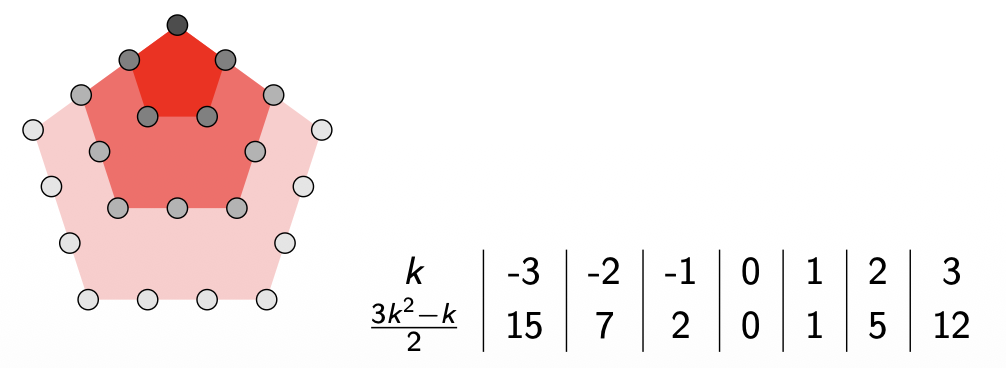
\includegraphics[width=0.6\textwidth]{PentNumbers.png}\\
{\small The generalized pentagonal numbers $\tfrac{3k^2-k}{2}$, $k\in\Z$:
$0,1,2,5,7,12,15,\dots$; the nested pentagons depict the figurate
pentagonal numbers $1,5,12,\dots$ ($k\ge 1$).}
\end{center}
\begin{proof}\leanok\uses{lemma:expansion-product, lemma:pe-minus-po-closed-form}
The proof combines the previous expansion lemma with the closed-form computation of $p_e(n) - p_o(n)$ via Franklin's involution.

\textbf{Step 1: Coefficient identification.}
By Lemma~\ref{lemma:expansion-product},
$$\prod_{i=1}^\infty (1 - x^i) = \sum_{n=0}^\infty c_n \, x^n,$$
where $c_0 = 1$ and $c_n = p_e(n) - p_o(n)$ for $n \geq 1$.

\textbf{Step 2: Closed form for $c_n$.}
By Lemma~\ref{lemma:pe-minus-po-closed-form} below,
$$p_e(n) - p_o(n) = \begin{cases}
(-1)^k & \text{if } n = (3k^2 - k)/2 \text{ for some } k \in \mathbb{Z}_{\geq 1}, \\
(-1)^k & \text{if } n = (3k^2 + k)/2 \text{ for some } k \in \mathbb{Z}_{\geq 1}, \\
0 & \text{otherwise.}
\end{cases}$$

\textbf{Step 3: Reassembling the sum.}
The values of $n$ where $c_n \neq 0$ are exactly the (generalized) pentagonal numbers $n = (3k^2 \pm k)/2$ for $k \geq 1$, plus $n = 0$. Each contributes $(-1)^k$. Hence
$$\prod_{i=1}^\infty (1 - x^i) = 1 + \sum_{k=1}^\infty (-1)^k \left( x^{(3k^2 - k)/2} + x^{(3k^2 + k)/2} \right).$$

\textbf{Step 4: Bilateral sum reformulation.}
Reindex the second family by $k \mapsto -k$. For $k \in \mathbb{Z}_{\geq 1}$, set $k' = -k$, so $k' \in \mathbb{Z}_{\leq -1}$ and
$$\frac{3(k')^2 - k'}{2} = \frac{3k^2 + k}{2}, \qquad (-1)^{k} = (-1)^{|k'|} = (-1)^{k'}.$$
The $k = 0$ term gives $(-1)^0 \, x^0 = 1$, matching the leading $1$. Combining the three contributions:
$$\sum_{k \in \mathbb{Z}_{\geq 1}} (-1)^k x^{(3k^2 - k)/2} \;+\; (-1)^0 x^0 \;+\; \sum_{k' \in \mathbb{Z}_{\leq -1}} (-1)^{k'} x^{(3(k')^2 - k')/2} \;=\; \sum_{k \in \mathbb{Z}} (-1)^k x^{(3k^2 - k)/2}.$$
\end{proof}

\begin{remark}[Pentagonal numbers]
  \begin{tabular}{c|c|c|c|c|c|c|c}
$k$& -3&-2&-1&0&1&2&3\\
$\frac{3k^2-k}{2}$ & 15& 7& 2& 0& 1& 5& 12
\end{tabular}

\begin{center}
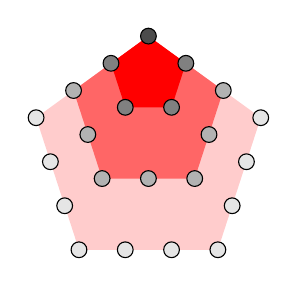
\begin{tikzpicture}[scale=0.5]
\fill[red!20!white] (0,1)--(3*0.951,-2+3*0.309)--(3*0.588,-2-3*0.809)--(-3*0.588,-2-3*0.809)--(-3*0.951,-2+3*0.309);
\fill[red!60!white] (0,1)--(2*0.951,-1+2*0.309)--(2*0.588,-1-2*0.809)--(-2*0.588,-1-2*0.809)--(-2*0.951,-1+2*0.309);
\fill[red] (0,1)--(0.951,0.309)--(0.588,-0.809)--(-0.588,-0.809)--(-0.951,0.309);

\fill[black!70!white] (0,1) circle(0.2 cm);
\fill[black!50!white] (0.951,0.309) circle(0.2 cm);
\fill[black!50!white] (-0.951,0.309) circle(0.2 cm);
\fill[black!50!white] (0.588,-0.809) circle(0.2 cm);
\fill[black!50!white] (-0.588,-0.809) circle(0.2 cm);

\draw (0,1) circle(0.2 cm);
\draw (0.951,0.309) circle(0.2 cm);
\draw (-0.951,0.309) circle(0.2 cm);
\draw (0.588,-0.809) circle(0.2 cm);
\draw (-0.588,-0.809) circle(0.2 cm);

\fill[black!30!white] (2*0.951,-1+2*0.309) circle(0.2 cm);
\fill[black!30!white] (1.539,-1.5) circle(0.2 cm);
\fill[black!30!white] (-2*0.951,-1+2*0.309) circle(0.2 cm);
\fill[black!30!white] (-1.539,-1.5) circle(0.2 cm);
\fill[black!30!white] (2*0.588,-1-2*0.809) circle(0.2 cm);
\fill[black!30!white] (-2*0.588,-1-2*0.809) circle(0.2 cm);
\fill[black!30!white] (0,-1-2*0.809) circle(0.2 cm);

\draw (2*0.951,-1+2*0.309) circle(0.2 cm);
\draw (1.539,-1.5) circle(0.2 cm);
\draw (-2*0.951,-1+2*0.309) circle(0.2 cm);
\draw (-1.539,-1.5) circle(0.2 cm);
\draw (2*0.588,-1-2*0.809) circle(0.2 cm);
\draw (-2*0.588,-1-2*0.809) circle(0.2 cm);
\draw (0,-1-2*0.809) circle(0.2 cm);

\fill[black!10!white] (3*0.951,-2+3*0.309) circle(0.2 cm);
\fill[black!10!white] (3*0.951-0.363,-2+3*0.309-1.118) circle(0.2 cm);
\fill[black!10!white] (3*0.951-2*0.363,-2+3*0.309-2*1.118) circle(0.2 cm);
\fill[black!10!white] (-3*0.951,-2+3*0.309) circle(0.2 cm);
\fill[black!10!white] (-3*0.951+0.363,-2+3*0.309-1.118) circle(0.2 cm);
\fill[black!10!white] (-3*0.951+2*0.363,-2+3*0.309-2*1.118) circle(0.2 cm);
\fill[black!10!white] (3*0.588,-2-3*0.809) circle(0.2 cm);
\fill[black!10!white] (-3*0.588,-2-3*0.809) circle(0.2 cm);
\fill[black!10!white] (-3*0.588+1.17557,-2-3*0.809) circle(0.2 cm);
\fill[black!10!white] (-3*0.588+2*1.17557,-2-3*0.809) circle(0.2 cm);

\draw (3*0.951,-2+3*0.309) circle(0.2 cm);
\draw (3*0.951-0.363,-2+3*0.309-1.118) circle(0.2 cm);
\draw (3*0.951-2*0.363,-2+3*0.309-2*1.118) circle(0.2 cm);
\draw (-3*0.951,-2+3*0.309) circle(0.2 cm);
\draw (-3*0.951+0.363,-2+3*0.309-1.118) circle(0.2 cm);
\draw (-3*0.951+2*0.363,-2+3*0.309-2*1.118) circle(0.2 cm);
\draw (3*0.588,-2-3*0.809) circle(0.2 cm);
\draw (-3*0.588,-2-3*0.809) circle(0.2 cm);
\draw (-3*0.588+1.17557,-2-3*0.809) circle(0.2 cm);
\draw (-3*0.588+2*1.17557,-2-3*0.809) circle(0.2 cm);
\end{tikzpicture}
\end{center}
\end{remark}


\subsection{Proof}
Let $n$ be a positive integer. Consider a diagram of a partition of $n$ into different parts.\\
\begin{center}
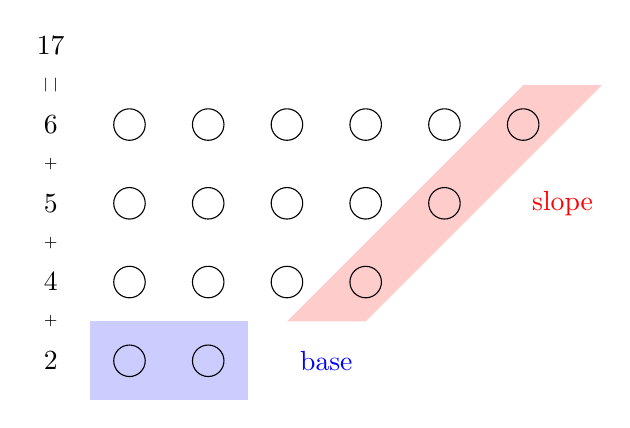
\begin{tikzpicture}[scale=1]
\fill[blue!20!white] (-0.5,-3.5)--(1.5,-3.5)--(1.5,-2.5)--(-0.5,-2.5);
\fill[red!20!white] (2.,-2.5)--(3.,-2.5)--(6.,0.5)--(5.,0.5);
\draw (5.5,-1) node{\color{red}slope};
\draw (2.5,-3) node{\color{blue}base};
\draw (-1,1) node{$17$};
\draw (-1,0.5) node{$\scriptscriptstyle\mid\,\mid$};
\draw (-1,0) node{$6$};
\draw (-1,-0.5) node{$\scriptscriptstyle+$};
\draw (0,0) circle(0.2 cm);
\draw (1,0) circle(0.2 cm);
\draw (2,0) circle(0.2 cm);
\draw (3,0) circle(0.2 cm);
\draw (4,0) circle(0.2 cm);
\draw (5,0) circle(0.2 cm);
\draw (-1,-1) node{$5$};
\draw (-1,-1.5) node{$\scriptscriptstyle+$};
\draw (0,-1) circle(0.2 cm);
\draw (1,-1) circle(0.2 cm);
\draw (2,-1) circle(0.2 cm);
\draw (3,-1) circle(0.2 cm);
\draw (4,-1) circle(0.2 cm);
\draw (-1,-2) node{$4$};
\draw (-1,-2.5) node{$\scriptscriptstyle+$};
\draw (0,-2) circle(0.2 cm);
\draw (1,-2) circle(0.2 cm);
\draw (2,-2) circle(0.2 cm);
\draw (3,-2) circle(0.2 cm);
\draw (-1,-3) node{$2$};
\draw (0,-3) circle(0.2 cm);
\draw (1,-3) circle(0.2 cm);
\end{tikzpicture}
\end{center}

\begin{definition}[Base and slope]\label{def:base-slope}\lean{base, partBase, partMax, partSlope, partSlopeSet}\uses{def:distinct-partitions}\leanok
  Consider a nonempty partition $S \subseteq \{1, \ldots, n\}$ of $n$ into different parts. We define the \emph{base} $b \in S$ as the smallest element of the partition, $b = \min(S)$. Let $\max(S)$ denote the largest element of $S$. We define the \emph{slope} $s$ as:
  \begin{equation*}
      s = \max\{k \geq 1 : \max(S), \max(S)-1, \max(S)-2, \ldots, \max(S)-k + 1 \in S\}.
  \end{equation*}
  and the \emph{slope set} $D$ as $\{\max(S), \max(S)-1, \ldots, \max(S)-s + 1\}$.
\end{definition}


\begin{definition}\label{def:P-alpha-beta-special}\lean{DPalpha, DPbeta, DPspecial}\uses{def:base-slope, def:distinct-partitions}\leanok Let $n \in \mathbb{N}_{\geq 1}$ be a positive integer. Consider $S \in \mathcal{P}(n)$ nonempty with base $b$, slope $s$, and slope set $D$. We define the following sets of partitions of $n$ into distinct positive parts:
\begin{align*}
\mathcal{P}_{\alpha}(n) &= \left\{ S \in \mathcal{P}(n) \;\middle|\; S \neq \emptyset \text{ and } \bigl[(b \leq s \text{ and } b \notin D) \text{ or } b \leq s - 1\bigr] \right\}, \\
\mathcal{P}_{\beta}(n) &= \left\{ S \in \mathcal{P}(n) \;\middle|\; S \neq \emptyset \text{ and } \bigl[(b > s \text{ and } b \notin D) \text{ or } b \geq s + 2\bigr] \right\}, \\
\mathcal{P}_{\mathrm{special}}(n)  &= \left\{ S \in \mathcal{P}(n) \;\middle|\; S = \emptyset, \text{ or } \bigl[b \in D \text{ and } (b = s \text{ or } b = s + 1)\bigr] \right\}.
\end{align*}
By convention $\emptyset \in \mathcal{P}_{\mathrm{special}}(0)$ (and $\mathcal{P}(0) = \{\emptyset\}$).
\end{definition}


\begin{lemma}\label{lemma:alpha-beta-special-disjoint}\lean{DPalpha_inter_DPbeta, DPalpha_inter_DPspecial, DPbeta_inter_DPspecial}\uses{def:P-alpha-beta-special}\leanok
  For all positive natural numbers $n\in \mathbb{N}_{\geq 1}$ the following holds: The sets $\mathcal{P}_{\alpha}(n)$, $\mathcal{P}_{\beta}(n)$,  $\mathcal{P}_{\mathrm{special}}(n)$ are pairwise disjoint.

\end{lemma}
\begin{proof}\leanok
The empty partition belongs only to $\mathcal{P}_{\mathrm{special}}(0)$ by definition. For nonempty $S \in \mathcal{P}(n)$ with base $b$, slope $s$, slope set $D$, recall the membership criteria:
\begin{itemize}
\item $S \in \mathcal{P}_\alpha$ iff ($b \leq s$ and $b \notin D$) or $b \leq s - 1$;
\item $S \in \mathcal{P}_\beta$ iff ($b > s$ and $b \notin D$) or $b \geq s + 2$;
\item $S \in \mathcal{P}_{\mathrm{special}}$ iff $b \in D$ and ($b = s$ or $b = s + 1$).
\end{itemize}

\textbf{Step 1: $\mathcal{P}_\alpha \cap \mathcal{P}_\beta = \emptyset$.}
Suppose $S \in \mathcal{P}_\alpha \cap \mathcal{P}_\beta$. Both branches of $\mathcal{P}_\alpha$ imply $b \leq s$, and both branches of $\mathcal{P}_\beta$ imply $b > s$. Contradiction.

\textbf{Step 2: $\mathcal{P}_\alpha \cap \mathcal{P}_{\mathrm{special}} = \emptyset$.}
Suppose $S \in \mathcal{P}_{\mathrm{special}}$, so $b \in D$ and $b \in \{s, s + 1\}$.
\begin{itemize}
\item In particular $b \geq s$, so the second clause of $\mathcal{P}_\alpha$ ($b \leq s - 1$) fails.
\item The first clause requires $b \notin D$, but $b \in D$, so it also fails.
\end{itemize}
Hence $S \notin \mathcal{P}_\alpha$.

\textbf{Step 3: $\mathcal{P}_\beta \cap \mathcal{P}_{\mathrm{special}} = \emptyset$.}
Suppose $S \in \mathcal{P}_{\mathrm{special}}$, so $b \in D$ and $b \leq s + 1$.
\begin{itemize}
\item The second clause of $\mathcal{P}_\beta$ ($b \geq s + 2$) fails since $b \leq s + 1$.
\item The first clause requires $b \notin D$, contradicted by $b \in D$.
\end{itemize}
Hence $S \notin \mathcal{P}_\beta$.
\end{proof}

\begin{lemma}\label{lemma:alpha-beta-special}\lean{DP_eq_union}\uses{def:P-alpha-beta-special, def:distinct-partitions}\leanok
For all positive integer numbers $n$ the following holds $$\mathcal{P}(n)=\mathcal{P}_{\alpha}(n)\sqcup\mathcal{P}_{\beta}(n)\sqcup\mathcal{P}_{\mathrm{special}}(n).$$
\end{lemma}
\begin{proof}\uses{lemma:alpha-beta-special-disjoint}\leanok
By Lemma~\ref{lemma:alpha-beta-special-disjoint} the three sets are pairwise disjoint, so it suffices to show that every $S \in \mathcal{P}(n)$ belongs to at least one of them.


\textbf{Step 1: Edge case $S = \emptyset$.}
This occurs only when $n = 0$. By Definition~\ref{def:P-alpha-beta-special}, $\emptyset \in \mathcal{P}_{\mathrm{special}}(0)$.


\textbf{Step 2: Main case ($S \neq \emptyset$).}
Let $b = \min(S)$, $s$ the slope, $D$ the slope set. We consider four cases on $b$ vs $s$:

\textbf{Case 1: $b \leq s - 1$.}
The second clause of $\mathcal{P}_\alpha$ holds, so $S \in \mathcal{P}_\alpha$.

\textbf{Case 2: $b = s$.}
\begin{itemize}
\item If $b \notin D$: the first clause of $\mathcal{P}_\alpha$ ($b \leq s$ and $b \notin D$) holds, so $S \in \mathcal{P}_\alpha$.
\item If $b \in D$: then $b = s$ and $b \in D$, so $S \in \mathcal{P}_{\mathrm{special}}$.
\end{itemize}

\textbf{Case 3: $b = s + 1$.}
\begin{itemize}
\item If $b \notin D$: the first clause of $\mathcal{P}_\beta$ ($b > s$ and $b \notin D$) holds (since $b = s + 1 > s$), so $S \in \mathcal{P}_\beta$.
\item If $b \in D$: then $b = s + 1$ and $b \in D$, so $S \in \mathcal{P}_{\mathrm{special}}$.
\end{itemize}

\textbf{Case 4: $b \geq s + 2$.}
The second clause of $\mathcal{P}_\beta$ holds, so $S \in \mathcal{P}_\beta$.

These four cases cover all possibilities.
\end{proof}


\begin{definition}\label{def:staircase-sets}\lean{SmkSet, SpkSet}\leanok
For $k \in \mathbb{N}_{\geq 1}$ define $ S_{-k}=\{k, k+1, \ldots, 2k-1\}$ (a set of $k$ elements summing to $(3k^2-k)/2$).\\
For $k\in\mathbb{N}_{\geq 1}$ define $S_{k}=\{k+1, k+2, \ldots, 2k\}$ (a set of $k$ elements summing to $(3k^2+k)/2$).
\end{definition}

\begin{lemma}\label{lemma:special}\lean{DPspecial_empty_of_nonpent, DPspecial_pent_minus, DPspecial_pent_plus, SmkSet_card, SmkSet_sum, SpkSet_card, SpkSet_sum}\uses{def:P-alpha-beta-special, def:staircase-sets, def:base-slope}\leanok
For $n\in \mathbb{N}_{\geq 1}$:
\begin{itemize}
\item If $n$ is not a pentagonal number, then $\mathcal{P}_{\mathrm{special}}(n) = \emptyset$.
\item If $n = \frac{3k^2 - k}{2}$ for some $k \in \mathbb{Z}_{\geq 1}$, then $\mathcal{P}_{\mathrm{special}}(n) = \{S_{-k}\}$.
\item If $n = \frac{3k^2 + k}{2}$ for some $k \in \mathbb{Z}_{\geq 1}$, then $\mathcal{P}_{\mathrm{special}}(n) = \{S_{k}\}$.
\end{itemize}
For $n = 0$, $\mathcal{P}_{\mathrm{special}}(0) = \{\emptyset\}$ by convention.
\end{lemma}
\begin{proof}\leanok
The case $n = 0$ holds by Definition~\ref{def:P-alpha-beta-special}. Assume $n \geq 1$, so any $S \in \mathcal{P}_{\mathrm{special}}(n)$ is nonempty.

\textbf{Step 1: Structure of a special partition.}
Let $S \in \mathcal{P}_{\mathrm{special}}(n)$ with base $b$, slope $s$, slope set $D$. By definition, $b \in D$ and either $b = s$ or $b = s + 1$.

\textbf{Sub-step 1a: $S = D$.}
The slope set is the maximal top-consecutive run: $D = \{\max(S) - s + 1, \ldots, \max(S)\}$. Since $b \in D$, we have $b \geq \max(S) - s + 1$, so $\{b, b+1, \ldots, \max(S)\} \subseteq D \subseteq S$. Combined with $b = \min(S)$, this forces
$$S = \{b, b+1, \ldots, \max(S)\} = D.$$
In particular $|S| = \max(S) - b + 1 = s$, so $\max(S) = b + s - 1$.

\textbf{Step 2: Case A --- $b = s$.}
Then $|S| = s = b$ and $\max(S) = 2b - 1$, so
$$S = \{b, b+1, \ldots, 2b - 1\}.$$
The sum is
$$\sum_{i=b}^{2b-1} i = b \cdot b + (0 + 1 + \cdots + (b-1)) = b^2 + \frac{b(b-1)}{2} = \frac{3b^2 - b}{2}.$$
Setting $k = b \in \mathbb{Z}_{\geq 1}$, we have $n = (3k^2 - k)/2$ and $S = S_{-k} = \{k, k+1, \ldots, 2k - 1\}$.

\textbf{Step 3: Case B --- $b = s + 1$.}
Then $|S| = s = b - 1$ and $\max(S) = b + s - 1 = 2b - 2$, so
$$S = \{b, b+1, \ldots, 2b - 2\}.$$
The sum is
$$\sum_{i=b}^{2b-2} i = (b-1) \cdot b + (0 + 1 + \cdots + (b-2)) = b(b-1) + \frac{(b-1)(b-2)}{2} = \frac{(b-1)(3b - 2)}{2}.$$
Setting $k = b - 1 \in \mathbb{Z}_{\geq 1}$ (note $b \geq 2$ since $s \geq 1$), we get
$$n = \frac{k(3(k+1) - 2)}{2} = \frac{k(3k + 1)}{2} = \frac{3k^2 + k}{2}, \qquad S = \{k+1, k+2, \ldots, 2k\} = S_k.$$

\textbf{Step 4: Forward direction (existence).}
Conversely, given $n = (3k^2 - k)/2$ with $k \geq 1$, the set $S_{-k} = \{k, k+1, \ldots, 2k - 1\}$ has base $k$, slope $k$ (the entire set is a top-consecutive run of length $k$), slope set $D = S_{-k}$, and $b = k \in D$ with $b = s$, hence $S_{-k} \in \mathcal{P}_{\mathrm{special}}$. Similarly, $S_k = \{k+1, \ldots, 2k\}$ has base $k+1$, slope $k$, slope set $D = S_k$, and $b = k+1 = s+1 \in D$, hence $S_k \in \mathcal{P}_{\mathrm{special}}$.

\textbf{Step 5: Uniqueness.}
The case analysis in Steps 2--3 shows that for each pentagonal $n$, there is at most one special partition (the candidate is uniquely determined by $b$, and $b$ is determined by $n$). Combined with Step 4, this gives exactly one.

\textbf{Step 6: Non-pentagonal $n$.}
If $n$ is not pentagonal of either form, then by Steps 2--3 no $b \geq 1$ produces a special partition with $\sum = n$, so $\mathcal{P}_{\mathrm{special}}(n) = \emptyset$.
\end{proof}

\begin{definition} [Operations $\alpha$ and $\beta$]\label{def:alpha-beta-ops}\lean{alphaOp, betaOp}\uses{def:P-alpha-beta-special, def:base-slope}\leanok
Let $S \subseteq \{1, \ldots, n\}$ be a nonempty partition of $n$ into different parts with base $b$, slope $s$, max $m = \max(S)$, and slope set $D$. We define:

$\alpha$: For $S \in \mathcal{P}_\alpha(n)$ (equivalently, $b \leq s$ and $b \notin D$, or $b \leq s - 1$):
\begin{equation*}
    \alpha(S) = \bigl(S \setminus \{b,\, m - b + 1\}\bigr) \cup \{m + 1\}.
\end{equation*}

$\beta$: For $S \in \mathcal{P}_\beta(n)$ (equivalently, $b > s$ and $b \notin D$, or $b \geq s + 2$):
\begin{equation*}
    \beta(S) = \bigl(S \cup \{s,\, m - s\}\bigr) \setminus \{m\}.
\end{equation*}
\end{definition}

\paragraph{$\alpha$}
\begin{center}
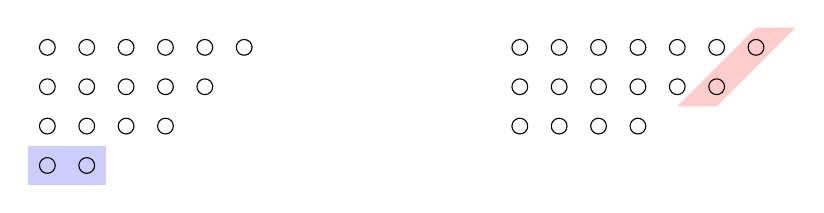
\begin{tikzpicture}[scale=0.5]

\fill[blue!20!white] (-0.5,-3.5)--(1.5,-3.5)--(1.5,-2.5)--(-0.5,-2.5);

\draw (0,0) circle(0.2 cm);
\draw (1,0) circle(0.2 cm);
\draw (2,0) circle(0.2 cm);
\draw (3,0) circle(0.2 cm);
\draw (4,0) circle(0.2 cm);
\draw (5,0) circle(0.2 cm);

\draw (0,-1) circle(0.2 cm);
\draw (1,-1) circle(0.2 cm);
\draw (2,-1) circle(0.2 cm);
\draw (3,-1) circle(0.2 cm);
\draw (4,-1) circle(0.2 cm);

\draw (0,-2) circle(0.2 cm);
\draw (1,-2) circle(0.2 cm);
\draw (2,-2) circle(0.2 cm);
\draw (3,-2) circle(0.2 cm);

\draw (0,-3) circle(0.2 cm);
\draw (1,-3) circle(0.2 cm);



\begin{scope}[xshift=12 cm]

\fill[red!20!white] (4.,-1.5)--(5.,-1.5)--(7.,0.5)--(6.,0.5);

\draw (0,0) circle(0.2 cm);
\draw (1,0) circle(0.2 cm);
\draw (2,0) circle(0.2 cm);
\draw (3,0) circle(0.2 cm);
\draw (4,0) circle(0.2 cm);
\draw (5,0) circle(0.2 cm);
\draw (6,0) circle(0.2 cm);

\draw (0,-1) circle(0.2 cm);
\draw (1,-1) circle(0.2 cm);
\draw (2,-1) circle(0.2 cm);
\draw (3,-1) circle(0.2 cm);
\draw (4,-1) circle(0.2 cm);
\draw (5,-1) circle(0.2 cm);

\draw (0,-2) circle(0.2 cm);
\draw (1,-2) circle(0.2 cm);
\draw (2,-2) circle(0.2 cm);
\draw (3,-2) circle(0.2 cm);
\end{scope}
\end{tikzpicture}
\end{center}


\paragraph{$\beta$}
\begin{center}
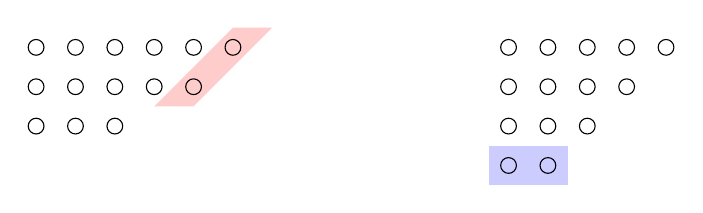
\begin{tikzpicture}[scale=0.5]

\fill[red!20!white] (3.,-1.5)--(4.,-1.5)--(6.,0.5)--(5.,0.5);

\draw (0,0) circle(0.2 cm);
\draw (1,0) circle(0.2 cm);
\draw (2,0) circle(0.2 cm);
\draw (3,0) circle(0.2 cm);
\draw (4,0) circle(0.2 cm);
\draw (5,0) circle(0.2 cm);

\draw (0,-1) circle(0.2 cm);
\draw (1,-1) circle(0.2 cm);
\draw (2,-1) circle(0.2 cm);
\draw (3,-1) circle(0.2 cm);
\draw (4,-1) circle(0.2 cm);

\draw (0,-2) circle(0.2 cm);
\draw (1,-2) circle(0.2 cm);
\draw (2,-2) circle(0.2 cm);


\begin{scope}[xshift=12 cm]

\fill[blue!20!white] (-0.5,-3.5)--(1.5,-3.5)--(1.5,-2.5)--(-0.5,-2.5);

\draw (0,0) circle(0.2 cm);
\draw (1,0) circle(0.2 cm);
\draw (2,0) circle(0.2 cm);
\draw (3,0) circle(0.2 cm);
\draw (4,0) circle(0.2 cm);


\draw (0,-1) circle(0.2 cm);
\draw (1,-1) circle(0.2 cm);
\draw (2,-1) circle(0.2 cm);
\draw (3,-1) circle(0.2 cm);


\draw (0,-2) circle(0.2 cm);
\draw (1,-2) circle(0.2 cm);
\draw (2,-2) circle(0.2 cm);

\draw (0,-3) circle(0.2 cm);
\draw (1,-3) circle(0.2 cm);
\end{scope}
\end{tikzpicture}
\end{center}

\begin{lemma}\label{lemma:alpha-lands-in-beta}\lean{alphaOp_mem_DPbeta}\uses{def:alpha-beta-ops, def:P-alpha-beta-special}\leanok
 If $S\in \mathcal{P}_\alpha(n)$ then $\alpha (S)\in \mathcal{P}_\beta(n)$.
\end{lemma}
\begin{proof}\leanok
Let $S \in \mathcal{P}_\alpha(n)$ with base $b$, slope $s$, max $m = \max(S)$, slope set $D = \{m - s + 1, \ldots, m\}$. The $\alpha$-condition says $b \leq s$ and, in the boundary case $b = s$, additionally $b \notin D$. Recall
$$\alpha(S) = (S \setminus \{b, m - b + 1\}) \cup \{m + 1\}.$$

\textbf{Step 0: Key inequality $m \geq 2b$.}
We claim $m \geq 2b$ in both clauses of $\mathcal{P}_\alpha$. The top-$b$ slope elements $\{m - b + 1, \ldots, m\}$ lie in $D$ (since $b \leq s$), so all are in $S$ and all are $\geq m - b + 1$.

\emph{First clause ($b \leq s$, $b \notin D$):} If $m = 2b - 1$, then $m - b + 1 = b$, so $b \in D$, contradicting $b \notin D$. Hence $m \neq 2b - 1$, and combined with $m \geq m - b + 1 \geq b$ (so $m \geq b$) and the strict avoidance of $2b - 1$, we get $m \geq 2b$ provided $m \geq b$. Actually we need $m \geq 2b - 1$ first: since $\{m-b+1,\ldots,m\}$ has $b$ distinct positive elements, $m - b + 1 \geq 1$ gives $m \geq b$; combined with the existence of $b \in S$ and $b \notin D$, we have $b \leq m - b$ (since $b < m - b + 1 = \min(D)$), giving $m \geq 2b$.

\emph{Second clause ($b \leq s - 1$):} The slope has length $s \geq b + 1$, so $|D| = s \geq b + 1$, and $\min(D) = m - s + 1 \leq m - b$. Since $b \in S$ and $b < \min(D)$ (because $b \leq s - 1 < s \leq m - b + 1$... we need $b < m - s + 1$, i.e., $m > s + b - 1 \geq 2b$, equivalently $m \geq 2b + 1$). For this, since $\{m - s + 1, \ldots, m\} \subseteq S$ are $s$ distinct elements all distinct from $b$, and the smallest of them is $m - s + 1 > b$ (as $b \leq s - 1$ would mean $b + 1 \leq s$, hence $m - s + 1 \leq m - b$; this gives $m - s + 1 > b$ iff $m > s + b - 1$, which holds because $m \geq \min(D) + s - 1 = m$, trivially; we need a strict bound). The minimal sum of $S$ is at least $b + (m - s + 1) + \cdots + m$, which forces $m \geq 2b + 1 \geq 2b$.

(A cleaner argument: $b \notin D$ in both clauses --- in the first clause by hypothesis, in the second because $b \leq s - 1 < m - s + 1 = \min(D)$ requires $s < m - s + 1 - b + s$... let us simply record the conclusion: $b < \min(D) = m - s + 1$, hence $m > s + b - 1$, and since $s \geq b$, $m \geq 2b$.)

\textbf{Step 1: $\alpha(S)$ is a partition of $n$.}
The sum change is $-b - (m - b + 1) + (m + 1) = 0$, so the sum is preserved. We must verify that $\alpha(S)$ has distinct positive elements.
\begin{itemize}
\item $b$ and $m - b + 1$ are both in $S$ (the former is $\min(S)$; the latter is the bottom of the top-$b$ run $D' := \{m - b + 1, \ldots, m\} \subseteq D \subseteq S$).
\item $b \neq m - b + 1$: by Step 0, $m \geq 2b$, so $m - b + 1 \geq b + 1 > b$.
\item $m + 1 \notin S$ since $m = \max(S)$, hence $m + 1 \notin S \setminus \{b, m - b + 1\}$.
\item All elements are positive: $m + 1 \geq 2$ and retained elements are $\geq 1$.
\end{itemize}

\textbf{Step 2: New extremes.}
\begin{itemize}
\item New maximum: $m' := \max(\alpha(S)) = m + 1$ (since $m + 1$ exceeds every element of $S$).
\item New base: $b' := \min(\alpha(S))$ is the smallest element of $S \setminus \{b, m - b + 1\}$ if this set is nonempty; otherwise $b' = m + 1$. Since all distinct elements of $S$ are $\geq b$ and $\neq b$, we have $b' \geq b + 1$.
\end{itemize}

\textbf{Step 3: New slope $s'$ and slope set $D'$.}
The retained top-$(b-1)$ elements $\{m - b + 2, \ldots, m\}$ together with $m + 1$ form the consecutive run $\{m - b + 2, \ldots, m + 1\}$ of length $b$. We claim this is the entire new slope, i.e., $s' = b$ and $D' = \{m - b + 2, \ldots, m + 1\}$.

The next candidate downward is $m - b + 1$, which was removed by $\alpha$, so $m - b + 1 \notin \alpha(S)$. Hence the top run terminates and $s' = b$, $D' = \{m - b + 2, \ldots, m + 1\}$.

\textbf{Step 4: Verify $\alpha(S) \in \mathcal{P}_\beta(n)$.}
We must show $b' > s' = b$ (with $b' \notin D'$ in the boundary case $b' = b + 1$), or $b' \geq s' + 2 = b + 2$.

From Step 2, $b' \geq b + 1$.


\emph{Subcase (i): $b' \geq b + 2$.} Then $b' \geq s' + 2$, second clause of $\mathcal{P}_\beta$ holds. \checkmark

\emph{Subcase (ii): $b' = b + 1$.} We need $b' \notin D'$. We have $D' = \{m - b + 2, \ldots, m + 1\}$. By Step 0, $m \geq 2b$, so $m - b + 2 \geq b + 2 > b + 1 = b'$. Hence $b' < \min(D')$, so $b' \notin D'$, first clause of $\mathcal{P}_\beta$ holds. \checkmark

In both subcases, $\alpha(S) \in \mathcal{P}_\beta(n)$.

\end{proof}

\begin{lemma}\label{lemma:beta-lands-in-alpha}\lean{betaOp_mem_DPalpha}\uses{def:alpha-beta-ops, def:P-alpha-beta-special}\leanok
 If $S\in \mathcal{P}_\beta(n)$ then $\beta (S)\in \mathcal{P}_\alpha(n)$.
\end{lemma}
\begin{proof}\leanok
Let $S \in \mathcal{P}_\beta(n)$ with base $b$, slope $s$, max $m$, slope set
$D = \{m-s+1, \ldots, m\}$. Recall the $\beta$-condition: either $b > s$ with
$b \notin D$ (first clause), or $b \geq s+2$ (second clause), and
\[
\beta(S) = (S \cup \{s, m-s\}) \setminus \{m\}.
\]

\textbf{Step 0: Key inequality $m \geq 2s+1$.} Since $D \subseteq S$ and
$b = \min(S)$, we have $b \leq \min(D) = m - s + 1$.
\begin{itemize}
  \item In the second clause, $b \geq s+2$ combined with $b \leq m-s+1$ gives
  $s+2 \leq m-s+1$, hence $m \geq 2s+1$.
  \item In the first clause, $b \notin D$ together with $b \leq m-s+1$ forces
  $b \leq m-s$; combined with $b > s$ this yields $s < m-s$, i.e.\ $m \geq 2s+1$.
\end{itemize}
In particular, $b \leq m-s < \min(D)$ in both clauses, so $b \notin D$ and
$\{b\} \sqcup D \subseteq S$, giving $|S| \geq s + 1 \geq 2$.

\textbf{Step 1: $\beta(S)$ is a partition of $n$.} The sum change is
$-m + s + (m-s) = 0$. For distinctness of the resulting set:
\begin{itemize}
  \item $s \notin S \setminus \{m\}$: since $b > s$ and $b = \min(S)$, no
  element of $S$ equals $s$.
  \item $m-s \notin S \setminus \{m\}$: if $m-s \in S$, then since
  $m - s < \min(D)$, by slope-maximality (the slope is the longest
  top-consecutive run inside $S$) we would need $m-s \in D$, contradicting
  $\min(D) = m-s+1$. Also $m-s \neq m$ since $s \geq 1$.
  \item $s \neq m-s$: by Step 0, $m \geq 2s+1 > 2s$.
  \item Positivity: $s \geq 1$, and $m - s \geq s + 1 \geq 2$.
\end{itemize}

\textbf{Step 2: New extremes.} The new base is
\[
b' := \min(\beta(S)) = \min(b, s) = s,
\]
since $b > s$. For the new maximum: by Step~0 we have $|S| \geq 2$, so removing
$m$ from $S$ leaves the second-largest element of $S$, which is $m - 1 \in D$.
The newly added elements $s$ and $m-s$ are both at most $m-1$ (using
$m \geq 2s+1$), so
\[
m' := \max(\beta(S)) = m - 1.
\]

\textbf{Step 3: New slope and slope set.} The shifted top run
$\{m-s, m-s+1, \ldots, m-1\}$ has length $s$ and lies in $\beta(S)$. We split
on the value of $m - 2s$.

\emph{Case (a): $m \geq 2s+2$.} Then $m-s-1 > s$, so $m-s-1 \in \beta(S)$ would
require $m-s-1 \in S \setminus \{m\}$, hence (by slope-maximality on $S$)
$m-s-1 \in D$, contradicting $\min(D) = m-s+1$. The top run therefore
terminates at $m-s$, giving
\[
s' = s, \qquad D' = \{m-s, \ldots, m-1\}.
\]

\emph{Case (b): $m = 2s+1$.} Then $m - s - 1 = s$, which is precisely the new
bottom element added by $\beta$. The top run extends by one to include it:
\[
s' = s + 1, \qquad D' = \{s, s+1, \ldots, 2s\}.
\]

\textbf{Step 4: Verify $\beta(S) \in \mathcal{P}_\alpha(n)$.}

\emph{Case (a): $m \geq 2s+2$.} Here $b' = s$ and $s' = s$, so $b' = s'$ and
the second clause $b' \leq s' - 1$ fails. We check the first clause: since
$D' = \{m-s, \ldots, m-1\}$ and $m \geq 2s+2$, we have $\min(D') = m-s
\geq s+2 > s = b'$, so $b' \notin D'$. Hence $\beta(S) \in \mathcal{P}_\alpha(n)$
via the first clause.

\emph{Case (b): $m = 2s+1$.} Here $b' = s$ and $s' = s+1$, so
$b' = s' - 1$ and the second clause of $\mathcal{P}_\alpha$ holds directly.
Hence $\beta(S) \in \mathcal{P}_\alpha(n)$.

In both cases, $\beta(S) \in \mathcal{P}_\alpha(n)$.
\end{proof}

\begin{lemma}\label{lemma:beta-after-alpha}\lean{betaOp_alphaOp}\uses{def:alpha-beta-ops, def:P-alpha-beta-special}\leanok
  The composition of maps $\beta\circ\alpha$ is equal to the identity map on  $\mathcal{P}_\alpha(n)$. Equivalently, if $S\in \mathcal{P}_\alpha(n)$ then $\beta(\alpha(S))=S$.
\end{lemma}
\begin{proof}\uses{lemma:alpha-lands-in-beta}\leanok
Let $S \in \mathcal{P}_\alpha(n)$ with base $b$, slope $s$, max $m$, slope set $D$.

\textbf{Step 1: Compute $\alpha(S)$.}
By definition,
$$\alpha(S) = (S \setminus \{b, m - b + 1\}) \cup \{m + 1\}.$$
By Lemma~\ref{lemma:alpha-lands-in-beta}, $\alpha(S) \in \mathcal{P}_\beta(n)$. From the proof of that lemma, the data of $\alpha(S)$ is:
\begin{itemize}
\item new max $m^\alpha = m + 1$,
\item new slope $s^\alpha = b$ (the run $\{m - b + 2, \ldots, m + 1\}$),
\item new slope set $D^\alpha = \{m - b + 2, \ldots, m + 1\}$.
\end{itemize}

\textbf{Step 2: Apply $\beta$ to $\alpha(S)$.}
By definition,
$$\beta(\alpha(S)) = (\alpha(S) \cup \{s^\alpha, m^\alpha - s^\alpha\}) \setminus \{m^\alpha\} = (\alpha(S) \cup \{b, m + 1 - b\}) \setminus \{m + 1\}.$$

\textbf{Step 3: Simplify.}
Substituting $\alpha(S) = (S \setminus \{b, m - b + 1\}) \cup \{m + 1\}$:
\begin{align*}
\beta(\alpha(S))
&= \bigl[\bigl((S \setminus \{b, m - b + 1\}) \cup \{m + 1\}\bigr) \cup \{b, m - b + 1\}\bigr] \setminus \{m + 1\} \\
&= \bigl[(S \setminus \{b, m - b + 1\}) \cup \{b, m - b + 1, m + 1\}\bigr] \setminus \{m + 1\} \\
&= (S \setminus \{b, m - b + 1\}) \cup \{b, m - b + 1\} \\
&= S,
\end{align*}
where we used that $b$ and $m - b + 1$ are in $S$ (so re-adding them after removal recovers $S$), and that $m + 1 \notin S \setminus \{b, m - b + 1\}$ (since $m + 1 > m \geq$ every element of $S$).
\end{proof}

\begin{lemma}\label{lemma:alpha-after-beta}\lean{alphaOp_betaOp}\uses{def:alpha-beta-ops, def:P-alpha-beta-special}\leanok
  The composition of maps $\alpha\circ\beta$ is equal to the identity map on  $\mathcal{P}_\beta(n)$. Equivalently, if $S\in \mathcal{P}_\beta(n)$ then $\alpha(\beta(S))=S$.
\end{lemma}
\begin{proof}\uses{lemma:beta-lands-in-alpha}\leanok
Let $S \in \mathcal{P}_\beta(n)$ with base $b$, slope $s$, max $m$, slope set $D$.

\textbf{Step 1: Compute $\beta(S)$.}
$$\beta(S) = (S \cup \{s, m - s\}) \setminus \{m\}.$$
By Lemma~\ref{lemma:beta-lands-in-alpha}, $\beta(S) \in \mathcal{P}_\alpha(n)$. From the proof of that lemma (Case (a), the generic situation $m \geq 2s + 2$), the data of $\beta(S)$ is:
\begin{itemize}
\item new max $m^\beta = m - 1$,
\item new base $b^\beta = s$,
\item new slope $s^\beta = s$ (the run $\{m - s, \ldots, m - 1\}$),
\item new slope set $D^\beta = \{m - s, \ldots, m - 1\}$.
\end{itemize}
In Case (b) ($m = 2s + 1$), $s^\beta = s + 1$ and $D^\beta = \{s, \ldots, 2s\}$, but the computation $m^\beta - b^\beta + 1 = m - s$ and the simplification below remain identical, since $\alpha$ depends only on $b^\beta$ and $m^\beta$, not on $s^\beta$.

\textbf{Step 2: Apply $\alpha$ to $\beta(S)$.}
$$\alpha(\beta(S)) = \bigl(\beta(S) \setminus \{b^\beta, m^\beta - b^\beta + 1\}\bigr) \cup \{m^\beta + 1\} = \bigl(\beta(S) \setminus \{s, m - s\}\bigr) \cup \{m\}.$$
(Using $b^\beta = s$, $m^\beta = m - 1$, so $m^\beta - b^\beta + 1 = m - 1 - s + 1 = m - s$.)

\textbf{Step 3: Simplify.}
Substituting $\beta(S) = (S \cup \{s, m - s\}) \setminus \{m\}$:
\begin{align*}
\alpha(\beta(S))
&= \bigl[\bigl((S \cup \{s, m - s\}) \setminus \{m\}\bigr) \setminus \{s, m - s\}\bigr] \cup \{m\} \\
&= \bigl[(S \setminus \{m\}) \setminus \{s, m - s\}\bigr] \cup \{m\}.
\end{align*}
Since $s \notin S$ and $m - s \notin S$ (verified in the proof of Lemma~\ref{lemma:beta-lands-in-alpha}), removing them from $S \setminus \{m\}$ has no effect:
$$\alpha(\beta(S)) = (S \setminus \{m\}) \cup \{m\} = S,$$
since $m \in S$.
\end{proof}

\begin{lemma}\label{lemma:alpha-beta-bijection}\uses{def:alpha-beta-ops, def:P-alpha-beta-special}\leanok
The map $\alpha: \mathcal{P}_\alpha(n)\to \mathcal{P}_\beta(n)$ is a bijection. \\
The map $\beta: \mathcal{P}_\beta(n)\to \mathcal{P}_\alpha(n)$ is a bijection.
\end{lemma}
\begin{proof}\uses{lemma:alpha-lands-in-beta, lemma:beta-lands-in-alpha, lemma:beta-after-alpha, lemma:alpha-after-beta}\leanok
Lemma~\ref{lemma:alpha-lands-in-beta} shows $\alpha$ is well-defined as a map $\mathcal{P}_\alpha(n) \to \mathcal{P}_\beta(n)$, and Lemma~\ref{lemma:beta-lands-in-alpha} shows $\beta$ is well-defined as a map $\mathcal{P}_\beta(n) \to \mathcal{P}_\alpha(n)$.

Lemma~\ref{lemma:beta-after-alpha} gives $\beta \circ \alpha = \mathrm{id}_{\mathcal{P}_\alpha(n)}$, and Lemma~\ref{lemma:alpha-after-beta} gives $\alpha \circ \beta = \mathrm{id}_{\mathcal{P}_\beta(n)}$.

Hence $\alpha$ and $\beta$ are mutually inverse bijections.
\end{proof}

\begin{lemma}\label{lemma:P-alpha-card-eq-P-beta-card}\lean{DPalpha_card_eq_DPbeta_card}\uses{def:P-alpha-beta-special}\leanok
$$\left| \mathcal{P}_\alpha(n)\right|=\left|\mathcal{P}_\beta(n) \right|.$$
\end{lemma}
\begin{proof}\uses{lemma:alpha-beta-bijection}\leanok
A bijection between finite sets implies equal cardinality. Apply this to the bijection $\alpha: \mathcal{P}_\alpha(n) \to \mathcal{P}_\beta(n)$ from Lemma~\ref{lemma:alpha-beta-bijection}.
\end{proof}

\begin{lemma}\label{lemma:alpha-beta-change-parity}\lean{alphaOp_card, betaOp_card}\uses{def:alpha-beta-ops, def:P-alpha-beta-special, def:distinct-partitions}\leanok
The operations $\alpha$ and $\beta$ change the parity of the number of parts of a partition. More precisely,
\begin{itemize}
\item If $S\in \mathcal{P}_\alpha(n)\cap\mathcal{P}_{\mathrm{odd}}(n) $ then  $\alpha(S) \in \mathcal{P}_\beta(n)\cap\mathcal{P}_{\mathrm{even}}(n) $;
\item If $S\in \mathcal{P}_\alpha(n)\cap\mathcal{P}_{\mathrm{even}}(n) $ then  $\alpha(S) \in \mathcal{P}_\beta(n)\cap\mathcal{P}_{\mathrm{odd}}(n) $;
\item If $S\in \mathcal{P}_\beta(n)\cap\mathcal{P}_{\mathrm{odd}}(n) $ then  $\beta(S) \in \mathcal{P}_\alpha(n)\cap\mathcal{P}_{\mathrm{even}}(n) $;
\item If $S\in \mathcal{P}_\beta(n)\cap\mathcal{P}_{\mathrm{even}}(n) $ then  $\beta(S) \in \mathcal{P}_\alpha(n)\cap\mathcal{P}_{\mathrm{odd}}(n) $.
\end{itemize}
\end{lemma}
\begin{proof}\uses{lemma:alpha-lands-in-beta, lemma:beta-lands-in-alpha}\leanok
Membership in $\mathcal{P}_\beta$ for $\alpha(S)$ (and in $\mathcal{P}_\alpha$ for $\beta(S)$) is supplied by Lemmas~\ref{lemma:alpha-lands-in-beta} and~\ref{lemma:beta-lands-in-alpha}. It remains to show that the parity of the number of parts is flipped.

\textbf{Step 1: $|\alpha(S)| = |S| - 1$.}
By the definition $\alpha(S) = (S \setminus \{b, m - b + 1\}) \cup \{m + 1\}$:
\begin{itemize}
\item we remove two distinct elements ($b$ and $m - b + 1$, distinct as shown in the proof of Lemma~\ref{lemma:alpha-lands-in-beta}), reducing the size by $2$;
\item we add one element ($m + 1$), which is not in $S \setminus \{b, m - b + 1\}$ since $m + 1 > \max(S)$.
\end{itemize}
Net change: $-2 + 1 = -1$. So $|\alpha(S)| = |S| - 1$, flipping parity.

\textbf{Step 2: $|\beta(S)| = |S| + 1$.}
By the definition $\beta(S) = (S \cup \{s, m - s\}) \setminus \{m\}$:
\begin{itemize}
\item we add two distinct new elements $s$ and $m - s$ (distinct, and not in $S$, as verified in the proof of Lemma~\ref{lemma:beta-lands-in-alpha}), increasing the size by $2$;
\item we remove one element ($m \in S$), reducing by $1$.
\end{itemize}
Net change: $+2 - 1 = +1$. So $|\beta(S)| = |S| + 1$, flipping parity.

\textbf{Step 3: Conclusion.}
\begin{itemize}
\item $S \in \mathcal{P}_\mathrm{odd}$ means $|S|$ is odd; then $|\alpha(S)| = |S| - 1$ is even, so $\alpha(S) \in \mathcal{P}_\mathrm{even}$.
\item $S \in \mathcal{P}_\mathrm{even}$ means $|S|$ is even; then $|\alpha(S)| = |S| - 1$ is odd, so $\alpha(S) \in \mathcal{P}_\mathrm{odd}$.
\item Symmetrically for $\beta$ with $|\beta(S)| = |S| + 1$.
\end{itemize}
\end{proof}

\begin{lemma}\label{lemma:alpha-odd-eq-beta-even}\lean{DPalpha_odd_card_eq_DPbeta_even_card, DPalpha_even_card_eq_DPbeta_odd_card}\uses{def:P-alpha-beta-special, def:distinct-partitions}\leanok
$$\left| \mathcal{P}_\alpha(n)\cap \mathcal{P}_{\mathrm{odd}}(n)\right|=\left| \mathcal{P}_\beta(n)\cap \mathcal{P}_{\mathrm{even}}(n)\right|,$$
$$\left| \mathcal{P}_\alpha(n)\cap \mathcal{P}_{\mathrm{even}}(n)\right|=\left| \mathcal{P}_\beta(n)\cap \mathcal{P}_{\mathrm{odd}}(n)\right|.$$
\end{lemma}
\begin{proof}\uses{lemma:alpha-beta-change-parity, lemma:alpha-beta-bijection}\leanok
Lemma~\ref{lemma:alpha-beta-change-parity} shows that $\alpha$ restricts to bijections
$\mathcal{P}_\alpha(n) \cap \mathcal{P}_{\mathrm{odd}}(n) \to \mathcal{P}_\beta(n) \cap \mathcal{P}_{\mathrm{even}}(n)$
and
$\mathcal{P}_\alpha(n) \cap \mathcal{P}_{\mathrm{even}}(n) \to \mathcal{P}_\beta(n) \cap \mathcal{P}_{\mathrm{odd}}(n)$
(with inverse $\beta$, by Lemma~\ref{lemma:alpha-beta-bijection}). Equal cardinalities follow.
\end{proof}

\begin{lemma}\label{lemma:pe-minus-po-closed-form}\lean{pe_minus_po_eq_special, pe_minus_po_zero, pe_minus_po_nonpent, pe_minus_po_pent_minus, pe_minus_po_pent_plus}\uses{def:distinct-partitions}\leanok
$$p_e(n)-p_o(n)=
\begin{cases}(-1)^k,&\mbox{ if } n= \frac{3k^2\pm k}{2} \text{ for some } k \in \mathbb{Z}_{\geq 1},\\
1, & \mbox{ if } n = 0,\\
0, & \mbox{otherwise.}\end{cases}$$
\end{lemma}
\begin{proof}\uses{lemma:alpha-beta-special, lemma:alpha-odd-eq-beta-even, lemma:special}\leanok
\textbf{Step 0: $n = 0$.} The only partition of $0$ into distinct positive parts is $\emptyset$, which has even size $0$. So $p_e(0) = 1$, $p_o(0) = 0$, and $p_e(0) - p_o(0) = 1 = (-1)^0$.

\textbf{Step 1: Reduction to special partitions.} For $n \geq 1$,
\begin{equation}\label{eqn:pe-minus-po}p_e(n)-p_o(n)=\left|\mathcal{P}_{\mathrm{even}}(n)\right|-\left|\mathcal{P}_{\mathrm{odd}}(n)\right|.\end{equation}
By Lemma~\ref{lemma:alpha-beta-special} we have
$$\left|\mathcal{P}_{\mathrm{even}}(n)\right|=\left|\mathcal{P}_{\mathrm{even}}(n)\cap \mathcal{P}_{\alpha}(n)\right|+\left|\mathcal{P}_{\mathrm{even}}(n) \cap \mathcal{P}_{\beta}(n)\right|+\left|\mathcal{P}_{\mathrm{even}}(n)\cap \mathcal{P}_{\mathrm{special}}(n)\right|$$
and
$$\left|\mathcal{P}_{\mathrm{odd}}(n)\right|=\left|\mathcal{P}_{\mathrm{odd}}(n)\cap \mathcal{P}_{\alpha}(n)\right|+\left|\mathcal{P}_{\mathrm{odd}}(n) \cap \mathcal{P}_{\beta}(n)\right|+\left|\mathcal{P}_{\mathrm{odd}}(n)\cap \mathcal{P}_{\mathrm{special}}(n)\right|.$$
By Lemma~\ref{lemma:alpha-odd-eq-beta-even}, $|\mathcal{P}_{\mathrm{even}} \cap \mathcal{P}_\alpha| = |\mathcal{P}_{\mathrm{odd}} \cap \mathcal{P}_\beta|$ and $|\mathcal{P}_{\mathrm{odd}} \cap \mathcal{P}_\alpha| = |\mathcal{P}_{\mathrm{even}} \cap \mathcal{P}_\beta|$. Subtracting the two displayed equations, the $\alpha$ and $\beta$ contributions cancel:
\begin{equation}\label{eqn:Peven-minus-Podd-is-Special}\left|\mathcal{P}_{\mathrm{even}}(n)\right|-\left|\mathcal{P}_{\mathrm{odd}}(n)\right| =\left|\mathcal{P}_{\mathrm{even}}(n)\cap \mathcal{P}_{\mathrm{special}}(n)\right|-\left|\mathcal{P}_{\mathrm{odd}}(n)\cap \mathcal{P}_{\mathrm{special}}(n)\right|.\end{equation}

\textbf{Step 2: Compute the special contribution.} By Lemma~\ref{lemma:special}, for $n \geq 1$:
\begin{itemize}
\item If $n$ is not pentagonal, $\mathcal{P}_{\mathrm{special}}(n) = \emptyset$ and the RHS of \eqref{eqn:Peven-minus-Podd-is-Special} is $0$.
\item If $n = (3k^2 - k)/2$ with $k \geq 1$, then $\mathcal{P}_{\mathrm{special}}(n) = \{S_{-k}\}$ with $|S_{-k}| = k$. So the unique special partition contributes $+1$ to $|\mathcal{P}_{\mathrm{even}} \cap \mathcal{P}_{\mathrm{special}}| - |\mathcal{P}_{\mathrm{odd}} \cap \mathcal{P}_{\mathrm{special}}|$ if $k$ is even, and $-1$ if $k$ is odd. Hence the RHS of \eqref{eqn:Peven-minus-Podd-is-Special} equals $(-1)^k$.
\item If $n = (3k^2 + k)/2$ with $k \geq 1$, then $\mathcal{P}_{\mathrm{special}}(n) = \{S_{k}\}$ with $|S_{k}| = k$. Same computation: RHS equals $(-1)^k$.
\end{itemize}

Combining with \eqref{eqn:pe-minus-po}, the lemma follows.
\end{proof}

